\chapter{软件实现与测试}

本章将从三个方面展示软件的实现成果与测试结果,分别是软件界面展示与功能测试、果实图像识别模型的训练结果以及针对核心接口的性能测试。

\section{软件功能测试与界面展示}\label{sec:test-func}

软件在一台 8G 内存、8核 CPU 的 MacOS 系统上成功运行。下面将对功能需求分析章节\ref{sec:req1}中提到的核心需求用例分别进行详细的用例测试,然后对其它基本功能给出最终的测试结果报告。

对提交称重数据需求用例\ref{tab:uc-weigh-submit}设计测试用例并进行测试,如表\ref{tab:uc-weigh-submit-test}所示。

\begin{longtable}[ht]{|c|p{8cm}|}
\caption{提交称重数据测试用例}
\label{tab:uc-weigh-submit-test}
\\
\hline
用例名称 & 提交称重数据 \\
\hline
用例描述 & 采摘员工在电子秤提交称重数据 \\
\hline
用例入口 & 电子秤提交称重数据 \\
\hline
测试步骤 & 1 运行电子秤模拟器 \\
& 2 点击生成数据 \\
& 3 点击识别果实 \\
& 4 点击提交数据 \\
\hline
测试用例 & 用例1 通过 MQTT 协议提交正常数据 \\
& 用例2 通过 CoAP 协议提交正常数据 \\
& 用例3 通过 STOMP 协议提交正常数据 \\
& 用例4 通过 HTTP 协议提交正常数据 \\
& 用例6 通过 MQTT 协议提交异常数据(不存在的电子秤, 编号为999) \\
& 用例7 通过 MQTT 协议提交异常数据(未启用的电子秤, 电子秤编号为1) \\
& 用例8 通过 MQTT 协议提交异常数据(不存在的果实, 果实编号为999) \\
& 用例9 通过 MQTT 协议提交异常数据(未启用的果实, 果实编号为1) \\
\hline
& 用例10 通过 MQTT 协议提交异常数据(不存在的采摘作业,果实编号为3) \\
& 用例11 通过 MQTT 协议提交异常数据(未开始或已结束的采摘作业,作业编号为4) \\
\hline
预期结果与实际结果 & 用例1:预期返回"成功",实际结果一致 \\
& 用例2:预期返回"成功",实际结果一致 \\
& 用例3:预期返回"成功",实际结果一致 \\
& 用例4:预期返回"成功",实际结果一致 \\
& 用例5:预期返回"成功",实际结果一致 \\
& 用例6:预期返回"失败",实际结果一致 \\
& 用例7:预期返回"失败",实际结果一致 \\
& 用例8:预期返回"失败",实际结果一致 \\
& 用例9:预期返回"失败",实际结果一致 \\
& 用例10:预期返回"失败",实际结果一致 \\
& 用例11:预期返回"失败",实际结果一致 \\
\hline
\end{longtable}

实际界面的测试结果如图\ref{fig:weigh-submit-result}所示。图中显示的是电子秤模拟器界面,包含9个输入框、4个操作按钮和1个结果显示区。

其中输入框包含通信协议(MQTT/HTTP/STOMP/CoAP)、电子秤编号、员工编号、果实编号、果实名称、果实图片、重量值、误差值和单位;提交按钮包含识别果实按钮、生成数据按钮、提交数据按钮和清除结果按钮;结果显示区包含记录编号、通信协议、作业编号、果实编号和提交结果。

\begin{figure}[H]
    \centering
    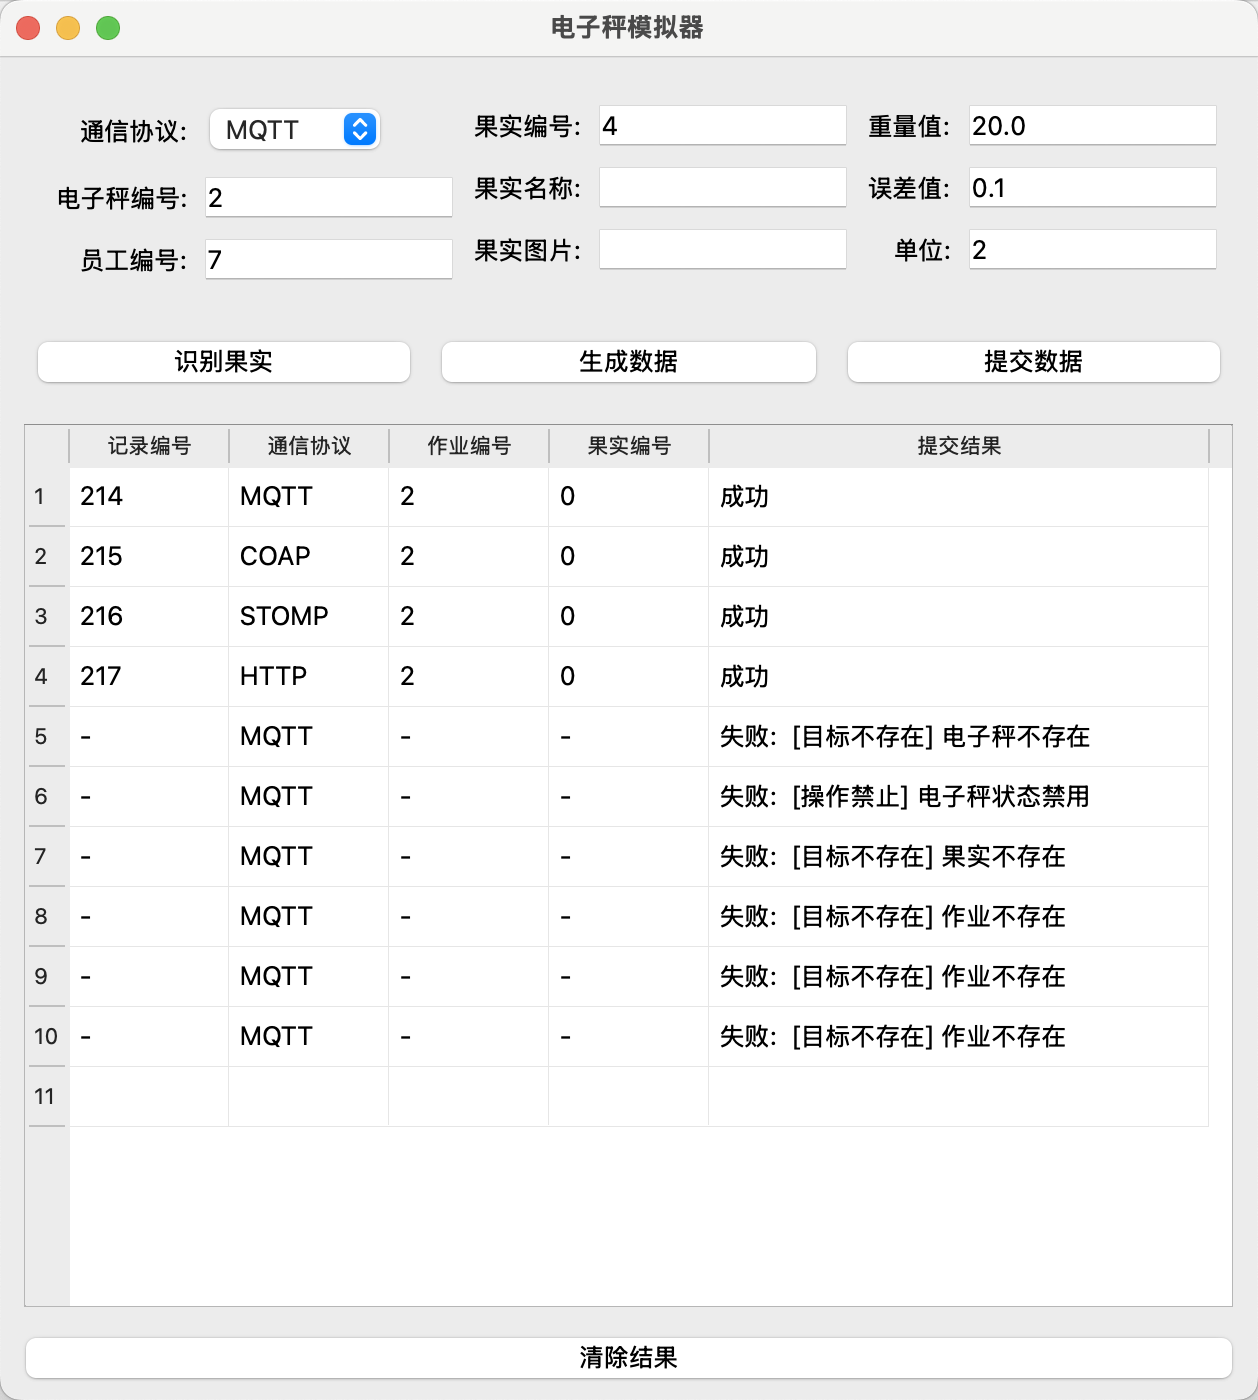
\includegraphics[width=0.8\linewidth]{../result/weigh-submit-result.png}
    \caption{提交称重数据用例测试截图}
    \label{fig:weigh-submit-result}
\end{figure}

对处理待办记录需求用例\ref{tab:uc-todo-handle}设计测试用例并进行测试,如表\ref{tab:uc-todo-handle-test}所示。

\begin{longtable}[ht]{|c|p{8cm}|}
\caption{处理待办记录测试用例}
\label{tab:uc-todo-handle-test}
\\
\hline
用例名称 & 处理待办记录 \\
\hline
用例描述 & 管理员在管理后台界面处理待办记录 \\
\hline
用例入口 & 后台管理界面中的待办管理模块 \\
\hline
测试步骤 & 1 点击提交待办 \\
& 2 选择果实种类 \\
& 3 点击确定,完成待办 \\
\hline
测试用例 & 用例1 提交正常数据 \\
& 用例2 提交异常数据(不存在的果实, 果实编号为999) \\
& 用例3 提交异常数据(未启用的果实, 果实编号为1) \\
\hline
预期结果与实际结果 & 用例1:预期返回"成功",实际结果一致 \\
& 用例2:预期返回"失败",实际结果一致 \\
& 用例3:预期返回"失败",实际结果一致 \\
\hline
\end{longtable}

实际界面的测试情况如图\ref{fig:todo-handle-result-1}和图\ref{fig:todo-handle-result-2}所示。

\begin{figure}[H]
    \centering
    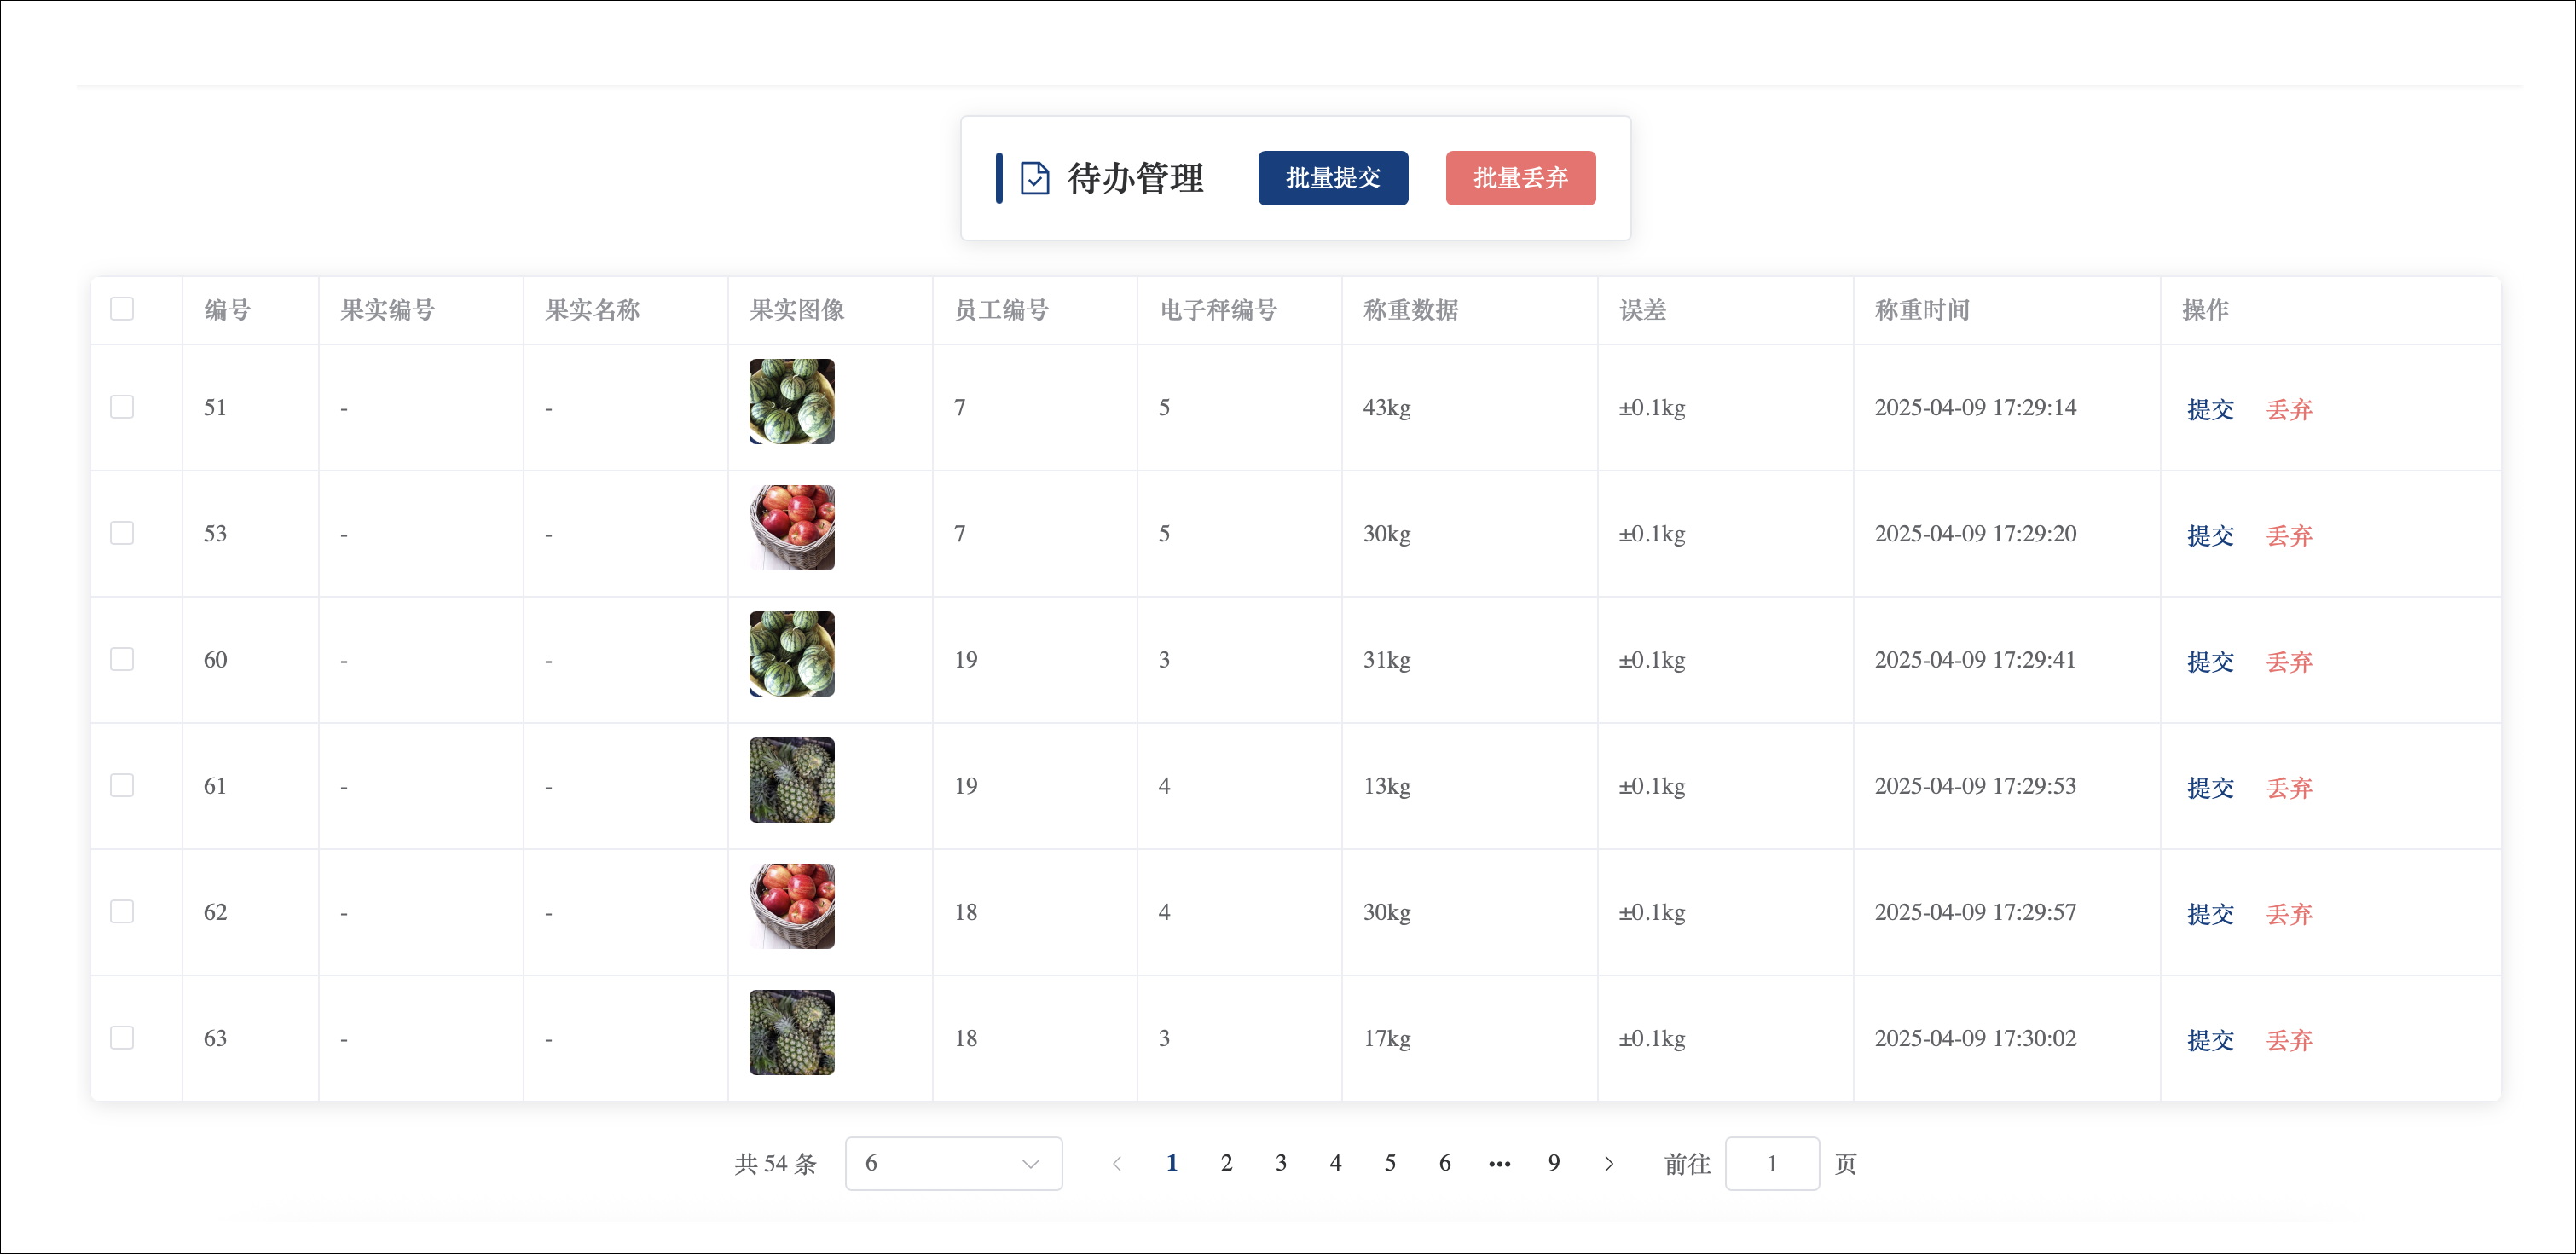
\includegraphics[width=0.8\linewidth]{../result/todo-handle-result-1.png}
    \caption{处理待办记录用例测试截图一}
    \label{fig:todo-handle-result-1}
\end{figure}

如图\ref{fig:todo-handle-result-1}所示,展现了软件管理后台中的待办管理界面,其中包含待办列表、4个操作按钮和分页块,其中待办列表表头包含编号、果实编号、果实名称、果实图像、员工编号、电子秤编号、称重数据、误差、称重时间和操作;操作按钮包含提交、丢弃、批量提交和批量丢弃。对某个待办项,点击提交按钮后,显示表单如图\ref{fig:todo-handle-result-2}所示。

\begin{figure}[H]
    \centering
    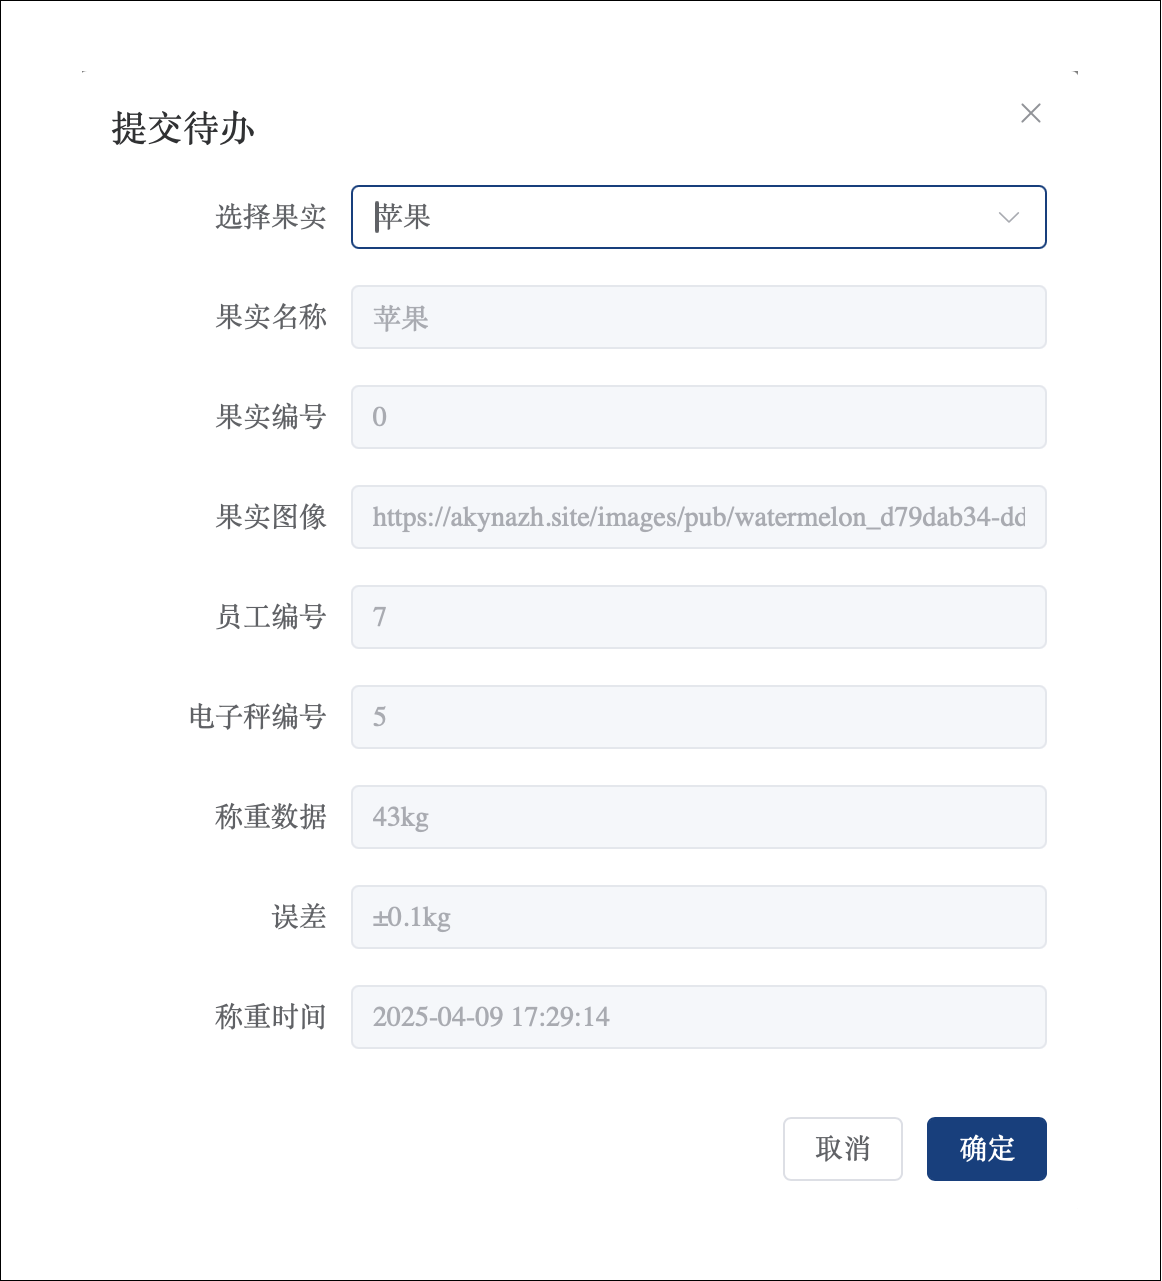
\includegraphics[width=0.8\linewidth]{../result/todo-handle-result-2.png}
    \caption{处理待办记录用例测试截图二}
    \label{fig:todo-handle-result-2}
\end{figure}

图\ref{fig:todo-handle-result-2}展现了待办项的提交表单,包含2个操作按钮和九个表单项,其中操作按钮包含取消和确认按钮;表单项包含选择果实、果实名称、果实编号、果实图像、员工编号、电子秤编号、称重数据、误差、称重时间,其中只能编辑果实,从选择果实项的下滑表单中选择果实后,果实名称和果实编号项将会随之变化。

对用户认证和授权需求用例\ref{tab:uc-user-auth}设计测试用例并进行测试,如表\ref{tab:uc-user-auth-test}所示。

\begin{longtable}[ht]{|c|p{8cm}|}
\caption{用户认证和授权测试用例}
\label{tab:uc-user-auth-test}
\\
\hline
用例名称 & xxx \\
\hline
用例描述 & xxx \\
\hline
用例入口 & xxx \\
\hline
测试步骤 & 1 xxx \\
& 2 xxx \\
& 3 xxx \\
\hline
测试用例 & 用例1 提交正常数据 \\
& 用例2 提交异常数据(xxx) \\
& 用例3 提交异常数据(xxx) \\
\hline
预期结果与实际结果 & 用例1:预期返回"成功",实际结果一致 \\
& 用例2:预期返回"失败",实际结果一致 \\
& 用例3:预期返回"失败",实际结果一致 \\
\hline
\end{longtable}

对果实图像识别需求用例\ref{tab:uc-produce-predict}设计测试用例并进行测试,如表\ref{tab:uc-produce-predict-test}所示。

\begin{longtable}[ht]{|c|p{8cm}|}
\caption{果实图像识别测试用例}
\label{tab:uc-produce-predict-test}
\\
\hline
用例名称 & xxx \\
\hline
用例描述 & xxx \\
\hline
用例入口 & xxx \\
\hline
测试步骤 & 1 xxx \\
& 2 xxx \\
& 3 xxx \\
\hline
测试用例 & 用例1 提交正常数据 \\
& 用例2 提交异常数据(xxx) \\
& 用例3 提交异常数据(xxx) \\
\hline
预期结果与实际结果 & 用例1:预期返回"成功",实际结果一致 \\
& 用例2:预期返回"失败",实际结果一致 \\
& 用例3:预期返回"失败",实际结果一致 \\
\hline
\end{longtable}

对新建采摘作业需求用例\ref{tab:uc-work-new}设计测试用例并进行测试,如表\ref{tab:uc-work-new-test}所示。

\begin{longtable}[ht]{|c|p{8cm}|}
\caption{新建采摘作业测试用例}
\label{tab:uc-work-new-test}
\\
\hline
用例名称 & xxx \\
\hline
用例描述 & xxx \\
\hline
用例入口 & xxx \\
\hline
测试步骤 & 1 xxx \\
& 2 xxx \\
& 3 xxx \\
\hline
测试用例 & 用例1 提交正常数据 \\
& 用例2 提交异常数据(xxx) \\
& 用例3 提交异常数据(xxx) \\
\hline
预期结果与实际结果 & 用例1:预期返回"成功",实际结果一致 \\
& 用例2:预期返回"失败",实际结果一致 \\
& 用例3:预期返回"失败",实际结果一致 \\
\hline
\end{longtable}

至此,完成对核心功能需求用例的设计与测试,下面给出对其它基本功能的测试结果报告,如表\ref{tab:test-result-summary}所示。

\begin{longtable}[ht]{|c|p{8cm}|c|}
\caption{基本功能测试结果报告}
\label{tab:test-result-summary}
\\
\hline
测试项 & 描述 & 测试结果 \\
\hline
用户管理 & 验证管理员添加、 & 正常 \\
\hline
\end{longtable}

\section{果实图像识别模型的训练结果}\label{sec:test-model}

农业果实称重云端软件基于 YOLOv8 实现果实图像识别功能,训练数据集来源于 Kaggle 平台上的已经完成数据标注的 Fruits-360 数据集。训练流程如下:

1、挑选来自 22 种不同果实的近三千张照片,将其上传至 Roboflow 平台;

2、在 Kaggle 云平台上,通过 Roboflow 提供的 API,将数据导出为 YOLOv8 格式的数据集;

3、使用 YOLOv8 模型训练数据集。训练进行 50 个 epoch,使用 yolov8m 预训练模型作为基础。训练过程中,如果验证集的性能在 30 个 epoch 内没有改进,训练将提前停止。

模型训练完成后,得到标准化混淆矩阵图如下:

\begin{figure}[H]
    \centering
    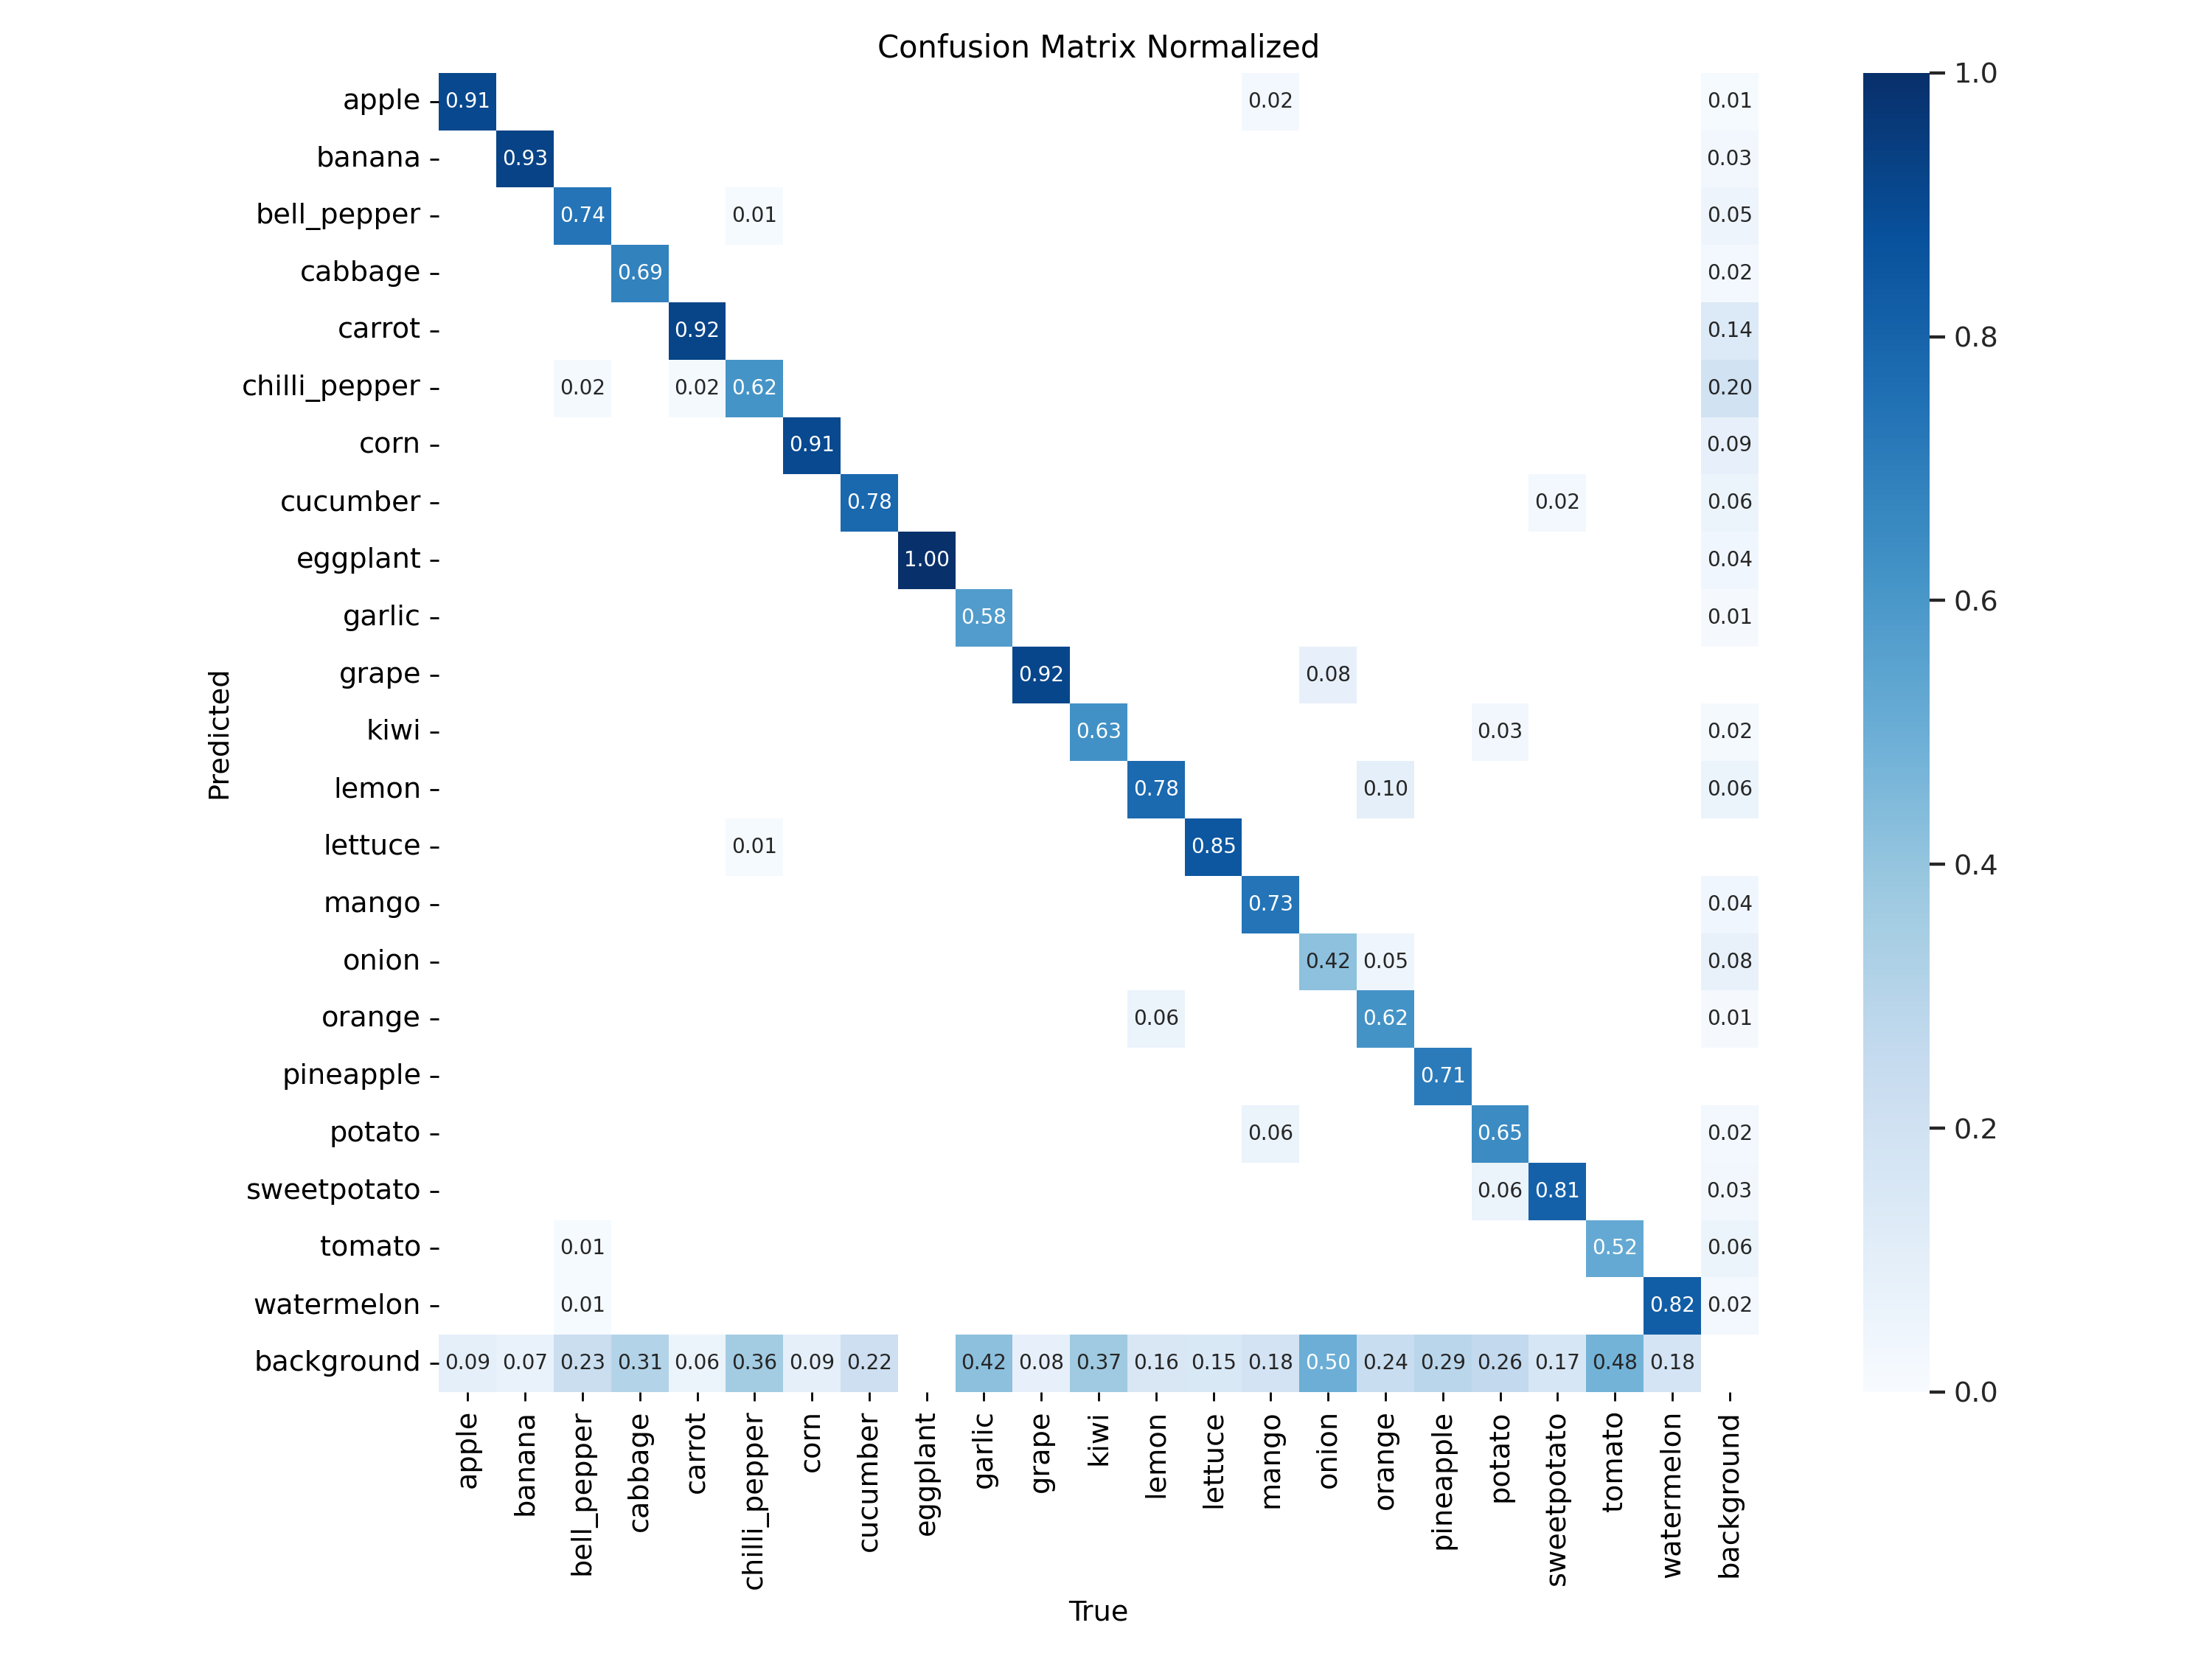
\includegraphics[width=0.8\linewidth]{../source/aws-img/yolov8/out/image/confusion_matrix_normalized.png}
    \caption{果实图像识别模型训练结果-标准化混淆矩阵图}
    \label{fig:confusion_matrix_normalized}
\end{figure}

从图\ref{fig:confusion_matrix_normalized}中的标准化混淆矩阵可以看出,模型在多个类别上表现出色。例如,apple(苹果)、banana(香蕉) 和 carrot(胡萝卜) 等类别的预测准确率都超过了 90\%,表明模型在这些类别上的预测非常精确。

然而,某些类别的分类效果较差,尤其是在 chilli\_pepper(辣椒) 和 background(背景) 类别上。chilli\_pepper 的准确率为 62\%,并且容易被误分类为 corn(玉米) 或其他类别。

此外,模型在识别 background 类别时的准确率较低,为 18\%,这可能是由于背景图像的多样性和噪声所致。

总体来说,模型在多数类别上的表现良好,但对于某些类别的混淆仍然存在,尤其是那些外观相似的类别(如 bell\_pepper(甜椒) 和 cabbage(白菜))。这种混淆可能来源于数据集中的样本不均衡、类别相似性较高或特征不足等问题。

\section{针对核心接口的性能测试}\label{sec:test-performance}

1、测试环境
2、测试用例
3、测试结果

\section{本章小结}